\section{Objetivos}

Em primeiro momento, o trabalho tem por objetivo fazer uma contextualização dos
métodos de cálculo e modelos utilizados, através de uma breve introdução
teórica. Contudo, o objetivo principal é avaliar a eficiência dos modelos de
atividade UNIFAC(Do) e F-SAC* na predição de valores da solubilidade de
antraceno em água. Para isso, serão feitas análises quali e quantitativa dos
resultados obtidos com o intuito de verificar qual dos modelos é mais adequado
para tal finalidade.

\section{Introdução Teórica}

\subsection{Modelo UNIFAC(Do)}

Segundo \citeonline{Fredenslund1975}, a metodologia UNIFAC (“Universal Quasi-chemical Functional Activity Coefficient”) pode ser utilizada para uma vasta quantidade de misturas exibindo desvios positivos ou
 negativos da lei de Raoult. O método UNIFAC segue o modelo “Analytical-
Solution-of-Groups”, ou ASOG, de \citeonline{Derr1969}, onde os coeficientes
 de atividade em misturas são relacionados às interações entre os grupos
 estruturais. Além disso, o método UNIFAC pode ser usado na previsão dos
 coeficientes de atividade para os componentes em misturas binárias desconhecidas que fazem parte de um determinado sistema multicomponentes, gerando, por exemplo, parâmetros binários em
 qualquer modelo de excesso de Gibbs.

\citeonline{Pollmann1996} afirmam que o logaritmo do coeficiente de atividade em uma mistura é calculado a partir da soma de duas contribuições. A primeira é denominada de combinatorial e refere-se aos diferentes tamanhos e formatos das moléculas. Já a segunda é chamada de residual, e representa a contribuição via interação energética entre
 as moléculas. A relação que descreve tal somatório está apresentada na
 \autoref{eq:001}:
\begin{equation}\label{eq:001}ln\gamma_i = ln\gamma_i^C +
ln\gamma_i^R\end{equation}
onde
$ln\gamma_i^C$ é o termo combinatório e $ln\gamma_i^R$ 
é o termo residual.

\citeonline{Muzenda2013} afirma que diferentes modificações foram propostas para os termos combinatorial e residual, bem como uma introdução da dependência da
 temperatura na interação dos parâmetros dos grupos funcionais. Publicado por \citeonline{Weidlich1987}, o UNIFAC(Dortmund) incorporou as seguintes características: utilização dos parâmetros de volume e área
 superficial de van der Waals para alcanos cíclicos e reclassificação dos álcoois em primário, secundário e terciário com seus próprios parâmetros
 de volume e área superficial de van der Waals; e a extensão do ajuste dos
 parâmetros de interação dos grupos funcionais para inclusão dos coeficientes de atividade à diluição infinita, equilíbrios líquido-vapor e entalpia em
 excesso, buscando aprimorar a precisão de tais parâmetros.

\citeonline{Jakob2006} cita que a parte combinatorial 
independente da temperatura é
calculada com os valores do volume via equação de van 
de Waals ($R_k$) e da área superficial ($Q_k$) dos grupos funcionais. 
Comparativamente com o modelo UNIFAC original, o UNIFAC(Do)
 apresenta uma mudança empírica na parte combinatorial ($V'$) 
para melhor descrever os sistemas assimétricos, como 
mostrado nas Equações \ref{eq:002} a \ref{eq:007}.

\begin{equation}\label{eq:002}
ln\gamma_i^C = 1 - V'_i + ln(V'_i) - 5q_i\left [ 1
- \frac{V_i}{F_i} + ln\left ( \frac{V_i}{F_i} \right ) \right ]
\end{equation}

\begin{equation}\label{eq:003}
V'_i = \frac{r_i^{3/4}}{\displaystyle\sum_jx_jr_j^{3/4}}
\end{equation}

\begin{equation}\label{eq:004}
V_i = \frac{r_i}{\displaystyle\sum_jx_jr_j}
\end{equation}

\begin{equation}\label{eq:005}
F_i = \frac{q_i}{\displaystyle\sum_jx_jr_j}
\end{equation}

O volume e área superficial relativos de van der Waals, para cada molécula $i$,
podem ser calculados pelas propriedades $R_k$  e $Q_k$  dos grupos estruturais
$k$ :

\begin{equation}\label{eq:006}
r_i = \displaystyle\sum_kv_k^{(i)}R_k
\end{equation}

\begin{equation}\label{eq:007}
q_i = \displaystyle\sum_kv_k^{(i)}Q_k
\end{equation}

A parte residual pode ser obtida utilizando os coeficientes de atividade dos
grupos funcionais $k$  na mistura ( $\Gamma_k$ ) e dos mesmos quando em uma
solução referência contendo apenas moléculas do tipo $i$ ( $\Gamma_k^{(i)}$ ):


\begin{equation}\label{eq:008}
ln\gamma_i^R = \displaystyle\sum_kv^{(i)}_k\left ( ln\Gamma_k -
ln\Gamma_k^{(i)} \right )
\end{equation}

A dependência da composição é expressa através do termo $\Gamma_k$, como
mostrado na \autoref{eq:009}:

\begin{equation}\label{eq:009}
ln\Gamma_k = Q_k\left ( 1 - ln\left ( \displaystyle\sum_m\Theta_m\Psi_{mk}
\right ) -
\displaystyle\sum_m\frac{\Theta_m\Psi_{km}}{\displaystyle\sum_n\Theta_n\Psi_{nm}}
\right )
\end{equation}
onde a fração de superfície ($\Theta_m$) e a fração molar ($X_m$) são definidas
nas Equações \ref{eq:010} e \ref{eq:011}.

\begin{equation}\label{eq:010}
\Theta_m = \frac{Q_mX_m}{\displaystyle\sum_nQ_nX_n}
\end{equation}

\begin{equation}\label{eq:011}
X_m =
\frac{\displaystyle\sum_jv^{(j)}_mx_j}{\displaystyle\sum_j\sum_nv_n^{(j)}x_j}
\end{equation}

A dependência da temperatura do parâmetro de interação entre os grupos
funcionais é descrita na \autoref{eq:012}, onde a interação é descrita entre os
grupos $n$ e $m$ .

\begin{equation}\label{eq:012}
\Psi_{nm} = exp \left ( \frac{-a_{nm} + b_{nm}T + c_{nm}T^2}{T} \right)
\end{equation}


\subsection{Modelo F-SAC*}

O modelo F-SAC calcula os coeficientes de atividade para a fase líquida via
\autoref{eq:001}.
O equacionamento dos termos combinatorial e residual, contudo, são apresentados nas 
Equações \ref{eq:013} e \ref{eq:014}. As relações quanto ao termo combinatorial
são semelhantes às mostradas para o UNIFAC(Do), mas o termo residual apresenta perfis de carga 
geradas pelos grupos funcionais presentes.

\begin{equation}\label{eq:013} 
ln\gamma_i^C = 1 - V'_i + ln(V'_i) - \frac{5q_i}{q}\left [ 1 
- \frac{V_i}{F_i} + ln\left ( \frac{V_i}{F_i} \right ) \right ] 
\end{equation}

\begin{equation}\label{eq:014} 
ln\gamma_i^R = \frac{\left( \Delta G_{i/s}^{*res} - \Delta
G_{i/i}^{*res} \right)}{RT}
\end{equation}
onde q é igual à 50 $\dot{A}^2$, $\Delta G_{i/s}^{*res}$ é a energia livre 
de Gibbs da carga ao redor da molécula de soluto na solução ($s$), 
$\Delta G_{i/s}^{*res}$ é a energia livre de Gibbs da carga no 
líquido puro ($i$), R é a constante universal dos gases e T a temperatura.

\citeonline{Soares2013} sugerem, no entanto, que a miscibilidade 
da mistura alcano-água pode ser melhor representada no modelo F-SAC 
se novos efeitos, ou parâmetros, fossem incomporados. Assim, 
\citeonline{Possani2014} introduziram a correção da temperatura 
para o termo eletrostático que é dependente do parâmetro que 
pareado entre os componentes da mistura ($\beta_{m,n}^{HB}$), 
ajustado a partir dos dados de temperaturas experimentais 
para cada caso. Além disso, quando tal parâmetro for nulo, 
o modelo retorna ao F-SAC original.

\section{Metodologia}

\subsection{Dados experimentais}

A \autoref{tab:dadosexp1_trab7} apresenta os dados de solubilidade do antraceno
em água para diferentes temperaturas. Nessa tabela, a solubilidade está sendo
expressa como sendo a fração molar de antraceno ($x_1$). Além disso, está
mostrado o logarítmo de $x_1$ e é com esse valor que serão construídos os
gráficos. Esse procedimento é realizado, pois os valores de solubilidade são
pequenos, e dessa forma, a análise da qualidade da predição dos modelos ficaria
prejudicada.

\clearpage

\begin{table}[htb]
\renewcommand{\arraystretch}{1.3}
\centering
\caption{Dados experimentais de solubilidade de antraceno ($x_1$) em água em
função da temperatura}
\begin{tabular}{S[table-format=6.6,round-mode=places,round-precision=0] S[table-format=6.6,round-mode=places,round-precision=2]S[table-format=6.6,round-mode=places,round-precision=3]}
\toprule
{$T (^\circ C)$}	&	{$x_1(\rm{x}10^{6})$} & {$\log(x_1)$}	\\
\midrule

120	&	1.59	&	-5.7986028757	\\
140	&	5.34	&	-5.272458743	\\
150	&	8.75	&	-5.057991947	\\
160	&	15.5	&	-4.8096683018	\\
180	&	52.9	&	-4.276544328	\\
200	&	153.0	&	-3.8153085692	\\

\bottomrule
\multicolumn{3}{c}{Fonte: Adaptado de \citeonline{Teoh2013}}
\end{tabular}
\label{tab:dadosexp1_trab7} 
\end{table} 

Para a realização dos cálculos, além da escolha de um modelo de atividade, são
necessários os valores de algumas propriedades do antraceno no ponto de fusão,
como a entalpia e temperatura. Os valores dessas grandezas estão mostrados na
\autoref{tab:dadosexp2_trab7}.

\begin{table}[htb]
\renewcommand{\arraystretch}{1.3}
\centering
\caption{Propriedades do antraceno: temperatura e entalpia de fusão}
\begin{tabular}{S[table-format=6.6,round-mode=places,round-precision=2]S[table-format=6.6,round-mode=places,round-precision=2]}
\toprule
{$T_{fus} (K)$}	&	{$\Delta H_{fus}(kJ/mol)$} \\
\midrule

489.4	&	28.8 \\

\bottomrule
\multicolumn{2}{c}{Fonte: Adaptado de \citeonline{Lisicki2000}}
\end{tabular}
\label{tab:dadosexp2_trab7} 
\end{table}

\subsection{Procedimento de cálculo}

Para o cálculo do equilíbrio sólido-líquido, partiu-se da definição da
igualdade de fugacidades, onde a fugacidade do componente $i$ da mistura é igual
em ambas as fases, como é mostrado abaixo:

\begin{equation}
\hat{f_i}^s = \hat{f_i}^l
\end{equation}

Contudo, partiu-se do pressuposto que o antraceno (componente 1) encontra-se
puro na fase sólida. Com isso, pode-se reescrever a equação anterior da seguinte
forma:

\begin{equation}
f_1^s = \hat{f_1}^l
\end{equation}

Através da definição de coeficiente de atividade, cujo valor pode ser
calculado pela razão da fugacidade do antraceno em mistura ($\hat{f_i}$) pela
sua fugacidade se estivesse em uma solução ideal $\left(\hat{f_i}^{Id}\right)$
, sendo a última obtida pelo produto da fração molar $x_1$ pela fugacidade do
antraceno puro ($f_i$), obtem-se:

\begin{equation}
f_1^s = x_1\gamma_1f_1^l
\end{equation}

Rearranjando a expressão e aplicando logarítmo dos dois lados da igualdade:

\begin{equation}\label{eq:ct7}
\ln \left( \frac{f_1^s}{f_1^l} \right) = \ln \left( x_1\gamma_1 \right)    
\end{equation}

Fazendo-se uma relação entre as energia livres de Gibbs em excesso do
antraceno nas fases sólida $\left(g_1^s\right)$ e líquida $\left(g_1^l\right)$ e
a fugacidade, chega-se na seguintes expressões apresentadas abaixo:

\begin{equation}\label{eq:at7}
g_1^s - g_1^l = RT\ln\left( \frac{f_1^s}{f_1^l} \right)   
\end{equation}

\begin{equation}\label{eq:bt7}
g_1^s - g_1^l = -\Delta g_{fus}  
\end{equation}

Substituindo as Equações \ref{eq:at7} e \ref{eq:bt7} na \autoref{eq:ct7}

\begin{equation}
\ln\left( x_1\gamma_1 \right) = \frac{-\Delta g_{fus}}{RT}
\end{equation}

Partindo da definição de energia livre de Gibbs em excesso $\left(g = h -
Ts\right)$, chega-se na seguinte expressão:

\begin{equation}\label{eq:gt7}
\ln\left( x_1\gamma_1 \right) = \frac{-\Delta h_{fus}}{RT} + \frac{\Delta
s_{fus}}{R}
\end{equation}

As variações de entalpia $\left( \Delta h_{fus,T} \right)$ e entropia
$\left(\Delta s_{fus,T}\right)$ de fusão em dada temperatura, em função destas
mesmas propriedades na temperatura de fusão $\left(T_{fus}\right)$, $\Delta
h_{fus,T_{fus}}$ e $\Delta s_{fus,T_{fus}}$, podem ser obtidas através das
seguintes expressões, em função da variação entre calores espercíficos do
antraceno sólido e líquido $\left(\Delta C_p^{sl}\right)$:

\begin{equation}\label{eq:dt7}
\Delta h_{fus,T} = \Delta h_{fus,T_{fus}} + \int_{T_{fus}}^{T}\Delta C_p^{sl}dT
\end{equation}

\begin{equation}\label{eq:et7}
\Delta s_{fus,T} = \Delta s_{fus,T_{fus}} + \int_{T_{fus}}^{T}\frac{\Delta
C_p^{sl}}{T}dT = \frac{\Delta h_{fus,T_{fus}}}{T_{fus}} + \int_{T_{fus}}^{T}\frac{\Delta
C_p^{sl}}{T}dT
\end{equation}

Simplificando as Equações \ref{eq:dt7} e  \ref{eq:et7} e substituindo na
\autoref{eq:gt7}, obtem-se a seguinte expressão:

\begin{equation}\label{eq:ft7}
\ln\left(x_1\gamma_1\right) =-\frac{\Delta
h_{fus,T_{fus}}}{R}\left[\frac{1}{T}-\frac{1}{T_{fus}}\right] -\frac{\Delta
C_p^{sl}}{R}\left[1-\frac{T_{fus}}{T}-\ln\left(\frac{T}{T_{fus}} \right)
\right]
\end{equation}

Contudo, muitas vezes não são encontrados dados de $C_p^{sl}$ disponíveis na
literatura, o que torna inviável a resolução da \autoref{eq:ft7}. Para contornas
essa situação, despreza-se o termpo que envolve o calor específicos e a expressão é
simplificada como apresentada a seguir:

\begin{equation}\label{eq:ht7}
\ln\left(x_1\gamma_1\right) = \frac{\Delta
h_{fus,T_{fus}}}{R}\left[\frac{1}{T_{fus}} - \frac{1}{T}\right]
\end{equation}

A \autoref{eq:ht7} será a expressão usada no presente trabalho para a predição
dos valores de solubilidade do antraceno em água.

\section{Resultados}

\subsection{Comparação entre valores de solubilidade: experimentais e
calculados}

A \autoref{fig:trab7a} apresenta um comparativo entre os valores logarítmos
calculados e experimentais de frações molares (solubilidade) de antraceno em
água. Os cálculos foram realizados utilizando F-SAC* e UNIFAC(Do) como modelos
de atividade. Ademais, a mesma apresenta uma região de tolerância (linhas tracejadas)
posicionada exatamente uma ordem de grandeza acima e abaixo da diagonal 
principal (linha contínua). Na diagonal principal, os valores calculados seriam
exatamente iguais aqueles experimentais. Portanto, quanto mais próximo os pontos
forem da diagonal, mais precisa é a prediação do modelo.

\clearpage
  
\begin{figure}
\centering
{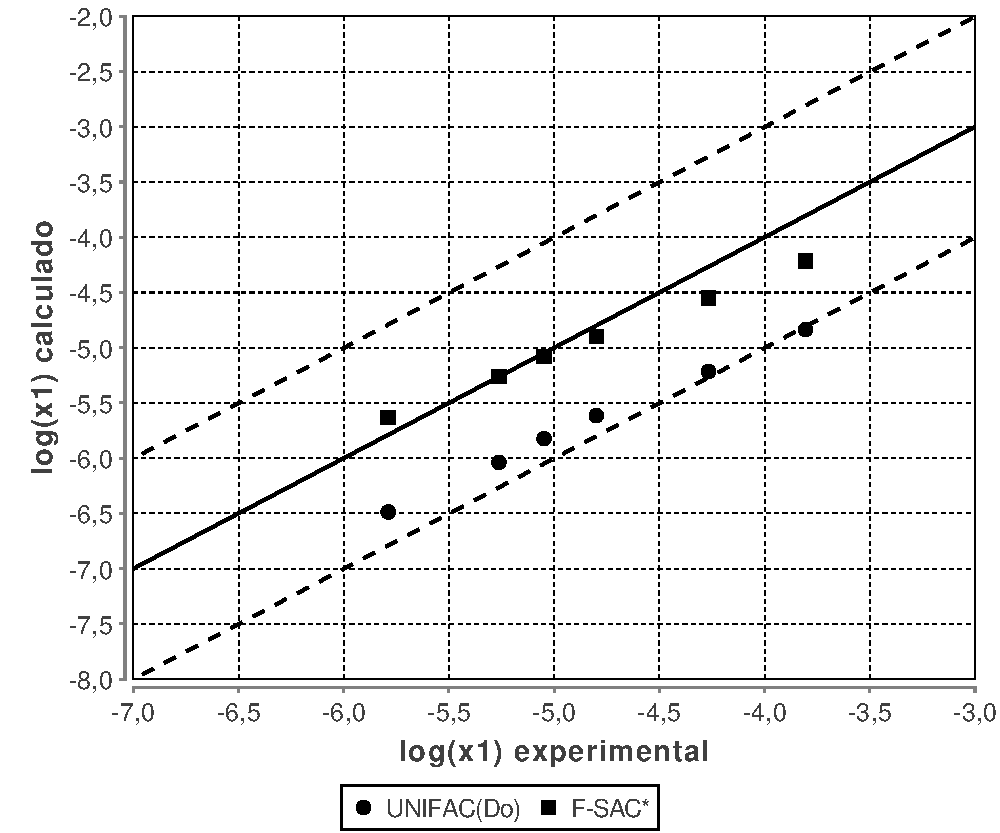
\includegraphics[width=0.8\textwidth]{img/trab7a.pdf}} 
\caption{Comparação entre as solubilidades calculadas e experimentais do
antraceno em água}
\label{fig:trab7a}
\end{figure}

Analisando os resultados da \autoref{fig:trab7a}, observa-se que os valores calculados
para o F-SAC* apresentam menor desvio, em relação ao diagonal principal, quando
comparados ao do UNIFAC(Do). A isso se deve o fato de que o F-SAC* é parametrizado 
para soluções de hidrocarbonetos em água. Embora este modelo (F-SAC*) 
não seja específico para equilíbrio sólido-líquido, é o que mais se aproxima 
do sistema estudado, pois, neste trabalho, fez-se a consideração da fase sólida 
como sendo antraceno puro.
	
	
\subsection{Comparação dos valores de calculados de solubilidade em função da
temperatura}
	
A \autoref{fig:trab7b} apresenta um comparativo entre os valores
calculados de solubilidade em função da temperatura. Nesta figura, a
solubilidade, como na \autoref{fig:trab7a}, é apresentada como logaritmo da
fração molar de antraceno. Os modelos são apresentados como diferentes linhas (
contínua para o UNIFAC(Do) e tracejada para o F-SAC*) e os dados experimentais
foram retirados da \autoref{tab:dadosexp1_trab7}.
\clearpage

\begin{figure}
\centering
{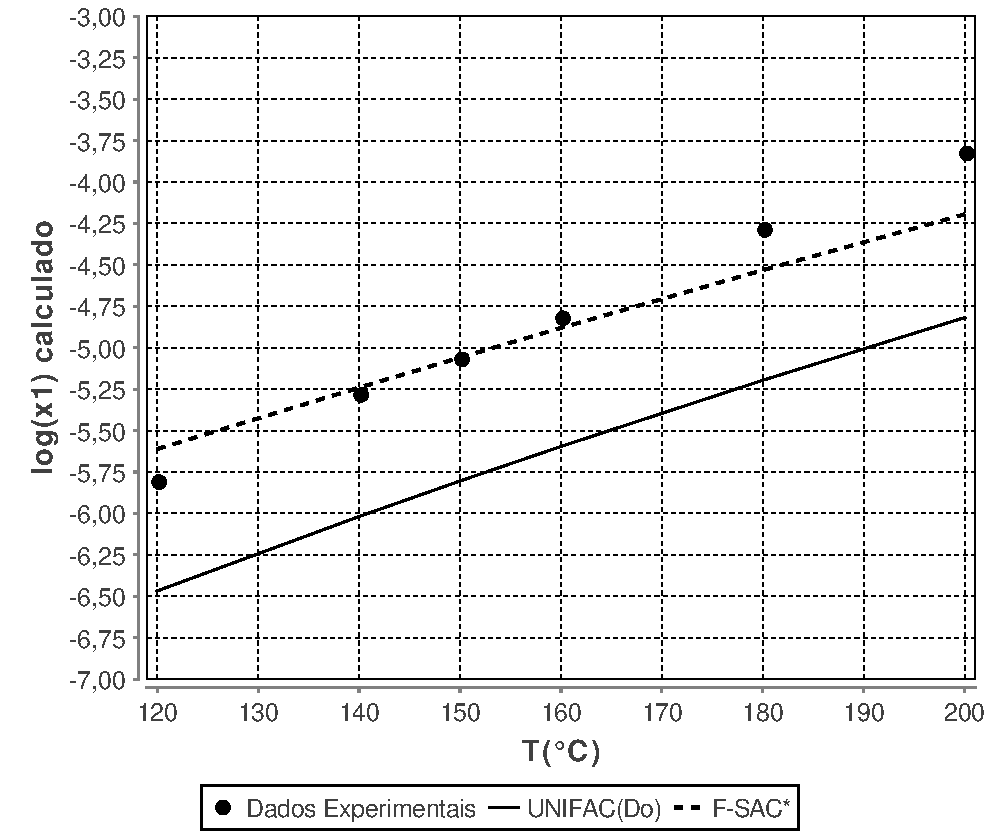
\includegraphics[width=0.8\textwidth]{img/trab7b.pdf}} 
\caption{Comparação entre as solubilidades calculadas e experimentais do
antraceno em água como função da temperatura}
\label{fig:trab7b}
\end{figure}

Observa-se, na \autoref{fig:trab7b}, para ambos os modelos, que a solubilidade
aumenta de acordo com o aumento da temperatura. Os valores calculados pelo F-SAC* 
apresentam desvio quantitativo menor que os calculados via UNIFAC(Do), 
todavia, seu erro qualitativo, ou seja, comparativo da inclinação da 
tendência dos pontos experimentais e o modelo, é mais significativo que 
aquele apresentado pelo UNIFAC(Do).
O modelo UNIFAC(Do), em toda a faixa de temperatura estudada, apresenta
valores de solubilidade subestimados, mantendo um desvio praticamente 
constante em relação aos pontos experimentais. Já o F-SAC*, superestima 
a solubilidade para baixas temperaturas e subestima quando para altas 
temperaturas e, além disso, observa-se que na região de 150 $^{\circ}$C , este
modelo a presenta erros quantitativos aproximadamente zerados.

\clearpage

\section{Conclusões}

Este trabalho visou comparar 2 diferentes modelos de atividade (UNIFAC(Do) 
e F-SAC*) na predição de um equilíbrio sólido-líquido para a mistura de 
antraceno e água. Foram utilizados dados experimentais retirados de
\citeonline{Teoh2013} e o software matemático $iiSE$ para calcular os coeficientes de atividade.
 
As Figuras \ref{fig:trab7a} e \ref{fig:trab7b} apresentam os resultados de
predição para ambos os modelos, comparando tais com os dados experimentais. 
Apesar dos melhores valores quantitativos do F-SAC*, o mesmo apresenta desvios 
qualitativos com relação aos pontos experimentais, observados através da
diferente inclinação entre tal tendência e o modelo. Assim, trata-se de um 
modelo cujo erro é regido pela temperatura, ou seja, há regiões de 
subestimação, superestimação e onde o erro é praticamente nulo.

Em contrapartida, o modelo UNIFAC(Do) apresenta erro quantitativos maiores, 
porém a tendência apresentada via erro qualitativo sempre remete a uma 
subestimação dos valores de solubilidade. Assim, os erros são sistemáticos,
remetendo a um maior conhecimento da predição para todos os pontos 
experimentais. Todavia, este modelo apresenta erros quantitativos cada vez
maiores com o aumento da temperatura.

